\documentclass[11pt, a4paper]{article}
\usepackage{multirow}
\usepackage{enumerate}
\usepackage{geometry}
\geometry{left=2.5cm,right=2.5cm,top=2.5cm,bottom=2.5cm}
%\usepackage{minted}
\usepackage[slantfont,boldfont]{xeCJK}
\setCJKmainfont{SimSun}
\usepackage{indentfirst}
\usepackage{float}
\setlength{\parindent}{2em}
\setCJKmonofont{SimHei}
\input zhwinfonts
\renewcommand\figurename{图}
\renewcommand\tablename{表}
\renewcommand\contentsname{\centering 目录}

\begin{document}
\title{{\bf\Huge 关于位图索引的若干问题及讨论} \\[2ex]{\huge 《算法设计与分析》课程第二次作业}}
  \author{计算机科学与技术学院\\马玉坤\\1150310618}
  \date{2017年5月9日}
  \maketitle

  \emph{在当今这个数据爆炸的时代,数据仓库的地位越来越重要。在众多数据仓库的实现方案中,位图索引与B树及其变种被广泛应用。本文讨论了位图索引领域部分极为重要的问题,并对前人的工作进行举例和比较。}\\
  {\bf 关键字:}位图索引,数据仓库,位图压缩,位图编码

  \tableofcontents

  \section{位图索引}

  位图索引 (Bitmap Index)由P’ONeil在1987年提出,并在一个商用数据库系统Model 204上首次应用。在数据库中,无论是用于科研用途,还是商业用途,位图向量都被广泛应用。\cite{art3}最原始的位图索引利用位向量 (Bit Vector)来表示某种被索引的属性在数据集中的索引情况。例如在表\ref{tb:table}中:在“数学成绩”一列中“优秀”这个属性的位图向量为101,分别代表小A拥有此属性、小B未拥有此属性,小C拥有此属性。将不同属性的位向量进行位逻辑运算,即可以响应各种复杂的(例如查询“语文成绩及格及以上且数学成绩及格及以上的人有哪些”)的数据库查询。

  \begin{table}[H]
    \centering
    \begin{tabular}{|l|l|l|}
      \hline
      姓名 & 数学成绩 & 语文成绩 \\ \hline
      小A & 优秀   & 及格   \\ \hline
      小B & 良好   & 优秀   \\ \hline
      小C & 优秀   & 不及格 \\ \hline
    \end{tabular}
    \label{tb:table} \caption{一个普通的数据库中的表}
  \end{table}

  \section{位图索引领域的相关问题}

  位图索引作为一种简单有效的数据库索引方式被广泛使用。有以下问题被广泛研究。

  \begin{enumerate}[1.]
  \item 对于单个位向量的压缩
  \item 对于整个位图索引的优化
  \item 位图索引的快速修改
  \end{enumerate}


  \subsection{对于单个位向量的压缩}

  对于一个位向量,例如''1000000100'',如何进行压缩也是一个热门的问题。如果能够对位图索引中的每个向量进行压缩,那么很多储存空间将会被节省,同时,查询效率也能得到提高。这对于数据量飞快增长的今天来说是至关重要的。\cite{art6}

  \subsection{位图索引的压缩}

  除了对于单个向量进行压缩,我们还可以考虑对于数据库中同一列的不同值对应的位向量进行整体压缩来减少储存空间并提高性能。例如,范围压缩是在值满足全序关系的列上可以使用的压缩方法。使用这种压缩方法,范围查询的效率将会大大提升。

  \subsection{位图索引的快速修改}

  位图索引尽管是被设计来高效地进行大量的数据库查询操作,但相对少量的数据库修改操作有时也是必要的。如何高效的能够让位图索引在能够进行高效查询的同时进行高效的修改,是数据库领域的热门问题。

  \section{对单个位向量的压缩}

  到目前为止,已经有众多有关压缩单个位向量的工作被做出。例如,通用的文字压缩算法,像LZ77,对于减少位向量存储大小十分有效,然而却并不能显著减少查询所需要消耗的时间,因为不同压缩后的位向量进行位操作前必须进行解压缩。对于位向量的压缩方法,通常使用的都是行程长度压缩 ({\bf RLE})方法,即将连续出现的相同的位合并,例如将11110000记做“4个连续的1+4个连续的0”。较为有名的行程长度压缩算法有BBC (Byte-aligned Bitmap Code)和WAH (Word-Alignment Hybrid Code)。

  \subsection{BBC (Byte-aligned Bitmap Code)}

  \begin{figure}[H]
    \begin{center}
      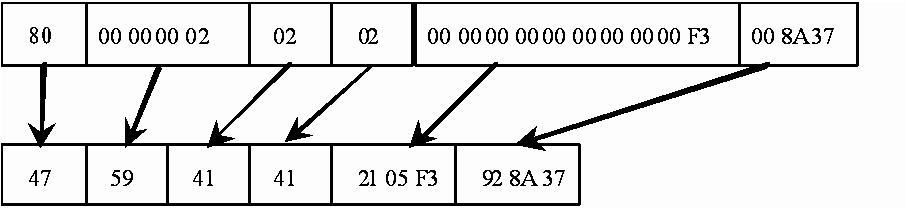
\includegraphics[width=5in]{bbc.png}
      \caption{BBC图解}\label{fig:bbc}
    \end{center}
  \end{figure}

  BBC将被压缩的位序列按字节分组为一系列节,压缩后的数据仍然以字节为单位。每节压缩后包括一个 fill 部分和一个 tail 部分。BBC中的字节包括两类:fill 字节和 literal 字节。fill 字节必须为全 1 或全 0,分别称为 1- fill 或 0- fill,literal 字节则按原文 (不压缩) 存放各位。单边 (One- sided) BBC只对 0- fill 压缩,适合于稀疏位图索引,双边 (Two- sided) 。BBC则对 0- fill 和 1- fill 均压缩。一个头字节 (Header byte) 用于表明节的种类。图\ref{fig:bbc}为一个位序列对应的 BBC压缩结果 (所有字节均用十六进制表示) 。

  \subsection{WAH (Word-Alignment Hybrid Code)}

  BBC以字节为单位进行位运算,然而计算机的 CPU 以字为单位进行位运算,所以 K. Wu 等人提出了以字为单位的位图索引编码:WAH。为了加快直接在压缩位图上的位运算速度,WAH 采用了更为简单的编码方式。WAH 中没有头字或头字节,这样就消除了压缩数据的前后依赖性,便于 CPU 并行处理。

  \begin{figure}[H]
    \begin{center}
      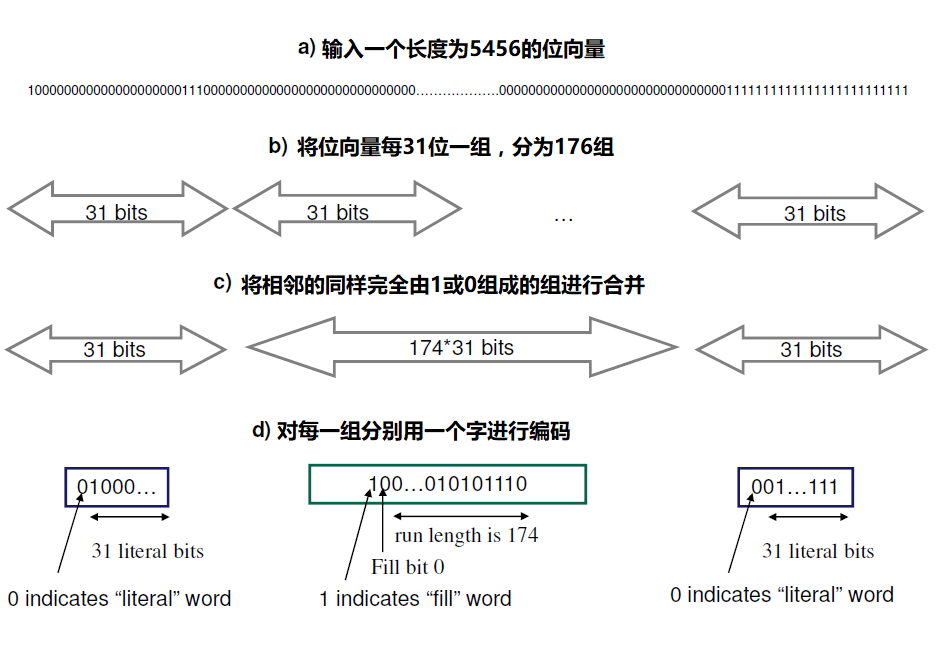
\includegraphics[width=5in]{wah.png}
      \caption{WAH图解}\label{fig:wah}
    \end{center}
  \end{figure}

  WAH 中只有两类字:literal 字和 fill 字,用最高位以示区别 (0 为 literal,1为 fill) 。令计算机的字长为 w,则 literal 字可保存 w- 1 个位。fill 字的次高位表示重复位是 0 还是 1,余下的 w-2 位则用于表示一个节的长度 (以字为单位) 。图\ref{fig:wah}表示一个位序列对应的 WAH 压缩结果。

  \subsection{BBC与WAH的比较}

  实际上,商业上的Oracle DBMS中就在使用BBC作为基本位图索引的压缩编码,鉴于Oracle DBMS的地位,这足以证明BBC的卓越性能。然而,许多实验表明WAH这种压缩方式在许多方面要比BBC有更好的性能。WAH使用空间换取了时间。在许多测试集上,平均情况下,WAH被测试要比BBC多使用50\%的空间,但速度比BBC快十倍。此外,更多的关于WAH的学术工作,已经能让使用WAH的位图索引的速度进一步提高。

  \section{对整个位图索引的优化}

  实际上,从一个完整的位图索引的角度来看,它的效率有极大的提升空间,因此学术界对于位图索引的空间效率与时间效率的优化进行了大量的研究。接下来我们将从占用空间、等值查询 (查询某列值=x) 效率、范围查询 (查询某列值<=x) 效率三个角度来分析各个位图索引实现方式的优劣。

  \subsection{基于编码 (Encoding) 的方法}

  \subsubsection{等值编码位图索引}

  等值编码位图索引是最基本的位图索引。它由$m$个位向量 $\{B_{m - 1}, B_{m-2}, \ldots, B_1, B_0\}$ 组成, 也可以看作一个 $n\times m$ 的矩阵, $B_j$ 是对应于属性值$j$的位向量, 当且仅当 $t_i.A =j$ 时, $B_j[i] =1$; 否则, $B_j[ i] =0$ 。图\ref{fig:column}表示一个有 10 个元组的表在 A 列上的投影 ($m=9$), 图\ref{fig:bitmap}为 A 列上的等值编码位图索引, 每一列代表一个位向量。

  \begin{figure}[H]
    \centering
      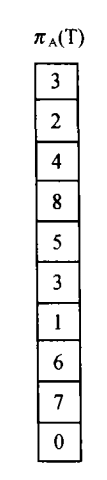
\includegraphics[width=0.8in]{column.png}
      \caption{数据库表中的一列}\label{fig:column}
  \end{figure}


  \begin{figure}[H]
    \centering
      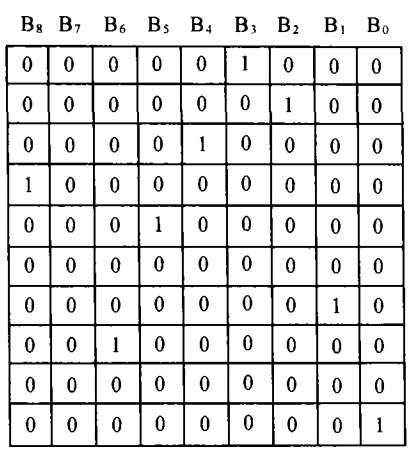
\includegraphics[width=3.5in]{bitmap.png}
      \caption{数据库表中某列对应的位图索引}\label{fig:bitmap}
  \end{figure}


  \subsubsection{范围编码位图索引}
  范围编码位图索引由$m-1$个位向量$\{B_{m-2}, B_{m-3}, \ldots, B_1,  B_0\}$组成, 其中 $B_j$ 对应于属性值 $j$, 当且仅当 $t_i.A \le j$ 时,$B_j[i] =1$。范围编码索引可以看作是等值编码位图索引的累积形式, 在等值编码位图索引中, 每一个位图向量对应于一个索引值, 而范围编码位图索引中, 每一位图向量代表所有小于等于对应值的索引值。 图\ref{fig:range}表示 A 上的范围编码位图索引。

  \begin{figure}[H]
    \centering
      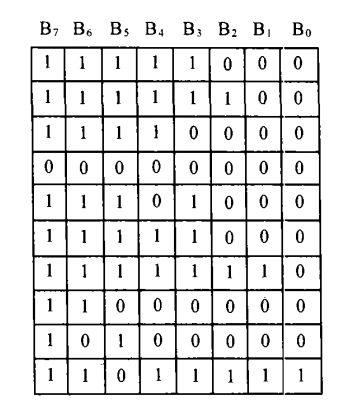
\includegraphics[width=3.5in]{range.png}
      \caption{数据库表中某列使用范围编码后的位图索引}\label{fig:range}
  \end{figure}

  \subsubsection{分段位图索引}

  分段位图索引由 Chan 和 I oannidis 提出,它将属性值用$r$进制表示。 在$r$进制中, 0到$m - 1$之间的每一个值$x$可以用长度为$e$的数字序列 ($x_{e-1}, …, x1, x0$) 表示, 其中 $e =「\log_m{r}」$、$0≤x_e, …, x_1 , x_0 <r$、$x = x_{e - 1} *r^{e-1} +…, + x_1 *r + x_0$。$e$位数字序列可以看成是$e$个列的值组成的, 相应的A列可划分成 e个子列$A_{e-1}, …, A_1, A_0$。 分段位图索引就是分别为每一个子列建立位图索引, 子列索引称为称为元索引, r为索引的基。 对于每一个元索引可以使用等值编码位图索引或范围编码位图索引。 对于\ref{fig:column}中的数据, A 列可以分裂为$A_1 、A_0$两个子列, 如图\ref{fig:base}所示。 图\ref{fig:base2}中的 (1) (2) 分别表示$A_1$、$A_0$的等值编码位图索引, 其中列$B^k_p$表示第$k$个元索引中对应于值$p$的位向量。图\ref{fig:base3}表示A列上以3为基的范围编码位图索引。

  \begin{figure}[H]
    \centering
    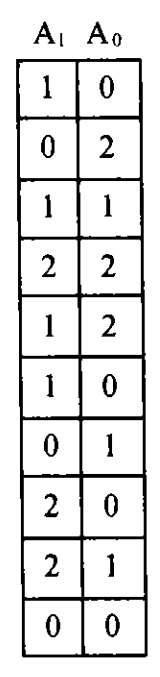
\includegraphics[width=0.9in]{base.png}
    \caption{列A以3为基分裂后的结果}\label{fig:base}
  \end{figure}
  \begin{figure}[H]
    \centering
    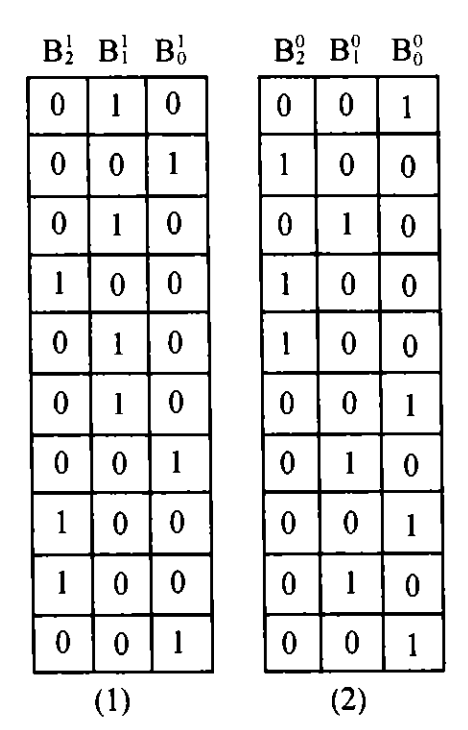
\includegraphics[width=2.5in]{base2.png}
    \caption{分段等值编码位图索引}\label{fig:base2}
  \end{figure}
  \begin{figure}[H]
    \centering
    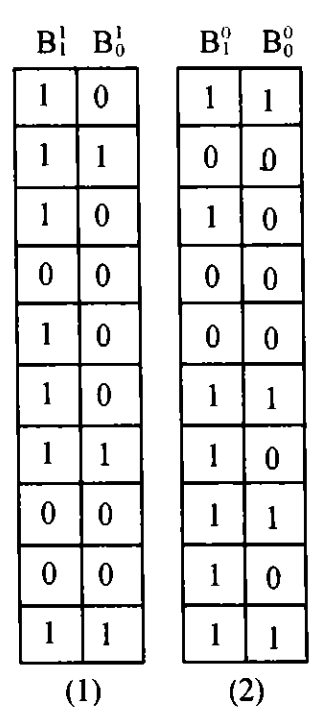
\includegraphics[width=1.75in]{base3.png}
    \caption{分段范围编码位图索引}\label{fig:base3}
  \end{figure}


  \subsection{基于分箱 (Binning) 的方法}

  该方法特别适用于有序属性 (如整数、实数等) 。首先,将被索引属性的取值分解为若干连续的区间,称为“箱”,然后位图索引针对每一个箱进行索引,从而显著减少了位图的数量。但基于分箱的位图索引对查询具有不稳定性,如果查询条件不是正好处在箱的边界,那么必须再次到边界箱对应的原始数据中检查数据是否符合查询条件,这一操作为称为“候选项检查 (Candidate Check) ”,其消耗的时间可能数倍于检索位图索引所需时间。对于图\ref{fig:binning}所示的分箱位图索引,若查询条件为“$37 \leq A < 63$”,需涉及箱 1、2、3,而箱 1 和 3 为边界箱,此时需要对箱 1 和箱 3 对应的位图中位为 1 的元组进行候选项检查,结果只有 61.7 符合查询条件。

  \begin{figure}[H]
    \centering
      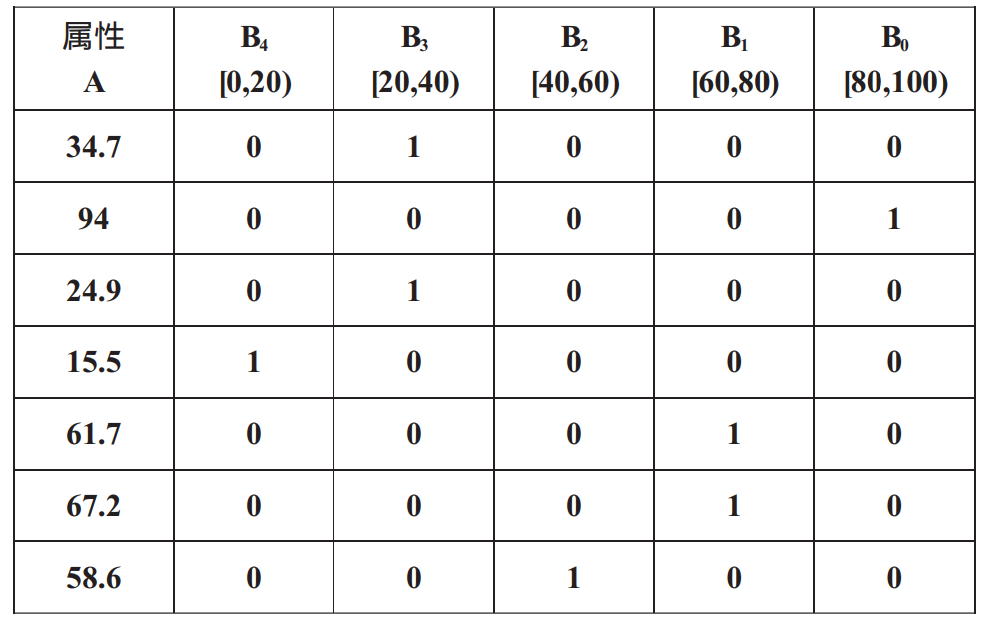
\includegraphics[width=5.5in]{binning.png}
      \caption{数据库表中某列使用范围编码后的位图索引}\label{fig:binning}
  \end{figure}

  \subsection{各种方法的比较}

  \begin{table}[H]
    \centering
    \begin{tabular}{|l|l|l|l|}
      \hline
      索引名称 & 占用空间 (向量数) & $A=x$的查询代价 & $A\leq x$的查询代价 \\
      \hline
      等值编码位图索引 & $m$ & 1 & $x$ \\
      \hline
      范围编码位图索引 & $m-1$ & 2 & $1$ \\
      \hline
      以r为基的等值编码位图索引 & $e*r$ & $e$ & $x_{e- 1} + … + x_1 + x_0$ \\
      \hline
      以 r 为基的范围编码位图索引 & $e*(r - 1)$ & $e*2$ & $2*(e - 1)+1$ \\
      \hline
      基于分箱的方法(箱数为K) & $m+K$ & $1$ & $\frac{m}{K} + K$\\
      \hline
    \end{tabular}
    \label{tb:table} \caption{一个普通的表}
  \end{table}


  \section{位图索引的快速修改}

  \subsection{Update Conscious Bitvector}

  UCB的主要思想如下:

  使用WAH\cite{art5}算法对位向量进行压缩后,压缩后的位向量上原地修改的效率堪忧,但是容易发现,在压缩后位向量的最后面添加一位的速度是极快的。对于可修改的位图向量的优化,一个直接想法是,既然修改操作并不多,原地修改的效率堪忧,为什么不把修改操作转化为禁用 (删除)+添加操作?这即是UCB (Update Conscious Bitmaps)的主要思想。\cite{art2}

  \begin{figure}[H]
    \centering
      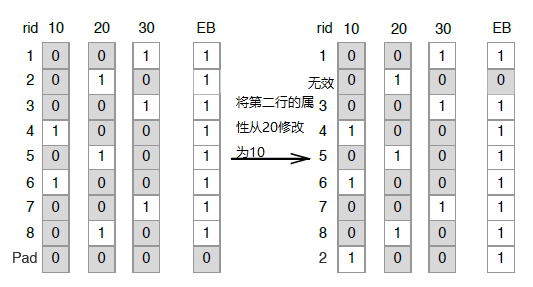
\includegraphics[width=5.5in]{ucb.png}
      \caption{UCB图解}\label{fig:ucb}
  \end{figure}

  在UCB中,每行都有一个额外的位向量叫做存在向量 (Existence Bitvector, EB)。当$EB_i$为1时,表示该行有效,否则该行无效(Invalid)。如图\ref{fig:ucb},当我们想要把第二行的值从20改为10时,我们只需要将$EB_2$设为0,然后在位向量后新建一位,并将对应的EB设为1。

  查询时,我们需要将对应的属性的位向量与存在向量进行“逻辑与”操作。

  \subsection{Upbit}

  UpBit并没有只使用一个存在向量,而是对每个属性都使用了一个更新向量(Update Bitvector,UB)。每一个属性的位向量,用两个位向量经“位异或”计算得出,这两个位向量分别为值向量 (Value Bitvector,VB)与更新向量 (Update Bitvector,UB)。\cite{art1}

  由于每一个属性的位向量用两个位向量经“位异或”计算得出。所以无论我们修改UB或者VB,都相当于对属性进行修改。在每次修改操作时,我们直接修改UB的值。如图\ref{fig:upbit},当我们想要把第二行的值从20修改为10,只需要把属性20对应的$UB_i$取反(从0变为1或者从1变为0),然后把属性10对应的$UB_i$取反。

  \begin{figure}[H]
    \begin{center}
      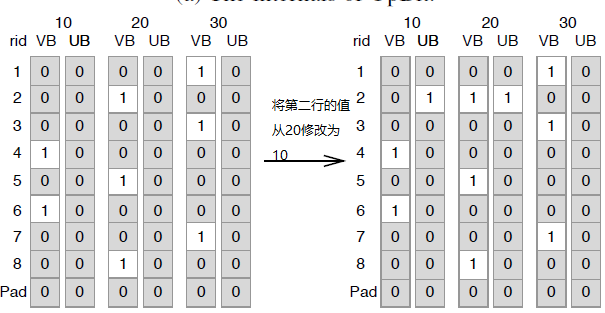
\includegraphics[width=5.5in]{upbit.png}
      \caption{Upbit图解}\label{fig:upbit}
    \end{center}
  \end{figure}

  \subsubsection{定时维护更新向量}

  当某个属性的UB的修改次数达到一定阈值时,我们将该属性的VB与UB做异或操作,将结果保存到VB中,然后将UB设为全0的向量,这便是对UB的维护。这样的维护可以保证随着修改操作积累,查询的效率仍然可以很快。

  \subsubsection{维护向量的分块指针}

  同时,UpBit还使用了第二种关键的提高效率的方法——块指针 (Fence Pointers)。当我们对某一行的值进行修改时,首先就需要找到这一行修改前的值。在寻找这一行修改前的值的过程中,我们需要在每一个属性的压缩后的UB和VB中查询这一行对应的二进制位的值。如何在压缩后的位向量中,快速找到第i位的值,是一个与效率关系极大的问题。块指针的思想是:将未压缩前的位向量按下标分为若干连续的块,每一块的块大小都接近g (g是人为给定的值)。对于每个位向量,维护每一块的起始位置对应的行在压缩后的位向量中的位置,就可以在$O(g+\log N/g)$的时间复杂度内快速在每个压缩后位向量中找到任意一行的位置,并可在$O(N/g)$的时间复杂度内维护修改后位向量的块指针。

  \subsection{两种方法的比较}

  实验中,UCB的确能极大地提高伴有少量修改操作的查询效率的提高,但是随着修改操作的积累,存在向量的复杂性将大大提高,UCB查询的效率将会极大地下降。然而Upbit对于这个问题并不敏感。

  无论是理论上,还是测试中,虽然Upbit使用的空间要比UCB大,但对于因为修改次数的积累造成的查询速度的下降并不敏感,所以效率要高很多。

  \section{总结}

  在现实中的应用场景下,综合地考虑各类算法,使得系统能够采取各个算法的长处,消除每个算法的短处。例如Multi-level以及Multi-component方法\cite{art6},综合使用各个不同的基于编码的位图向量,以获得更高的效率。

\renewcommand\refname{参考文献}
\begin{thebibliography}{99}
\bibitem{art1}Athanassoulis M, Yan Z, Idreos S. UpBit: Scalable In-Memory Updatable Bitmap Indexing[C]//Proceedings of the 2016 International Conference on Management of Data. ACM, 2016: 1319-1332.
\bibitem{art2}Canahuate G, Gibas M, Ferhatosmanoglu H. Update conscious bitmap indices[C]//Scientific and Statistical Database Management, 2007. SSBDM'07. 19th International Conference on. IEEE, 2007: 15-15.
\bibitem{art3}程鹏. 位图索引技术及其研究综述[J]. 科技信息, 2010 (26): 134-135.
\bibitem{art4}Wu K, Ahern S, Bethel E W, et al. FastBit: interactively searching massive data[C]//Journal of Physics: Conference Series. IOP Publishing, 2009, 180(1): 012053.
\bibitem{art5}Wu K, Otoo E J, Shoshani A. Compressing bitmap indexes for faster search operations[C]//Scientific and Statistical Database Management, 2002. Proceedings. 14th International Conference on. IEEE, 2002: 99-108.
\bibitem{art6}Madhu B. Multi-level and Multi-component Bitmap Encoding for Efficient Search Operations[J]. Database Systems Journal, 2012, III(4):47-60.

\end{thebibliography}

\end{document}
